\documentclass{article}

\usepackage[main,final]{neurips_2025}
\makeatletter\renewcommand{\@noticestring}{}\makeatother  % drop the conference footnote: this is a course report

\usepackage[utf8]{inputenc}
\usepackage[T1]{fontenc}
\usepackage{hyperref}
\usepackage{url}
\usepackage{booktabs}
\usepackage{amsmath, amssymb}
\usepackage{graphicx}
\usepackage{microtype}

\title{Convolutional VAEs for Chest X-ray Generation}

\author{%
  Vincent Chen \\
  ECE 285 Homework 1, UC San Diego \\
  \url{https://github.com/mao3267/ece285-hw1-vae-chest-xray}
}

\setlength{\abovecaptionskip}{3pt}
\setlength{\belowcaptionskip}{0pt}
\setlength{\textfloatsep}{8pt plus 2pt minus 2pt}
\setlength{\floatsep}{6pt plus 2pt minus 2pt}

\begin{document}

\maketitle
\vspace{-1.2em}

\begin{abstract}
We train convolutional VAEs on pediatric chest X-rays and score samples with FID and Inception Score. A sweep over the KL weight $\beta\in\{1,0.1,0.01\}$ shows that reconstructions improve as $\beta$ falls (FID 221 to 134), while prior samples improve only at $\beta{=}0.01$ (219, 220, 185). Sampling from a Gaussian mixture fitted to the training latents helps once $\beta$ is small and closes about half of the gap to reconstructions; the best model ($\beta{=}0.01$, mixture sampling) reaches FID 158. An ablation shows that rotation/translation augmentation hurts (FID 214), which we attribute to dark corner artifacts from the black fill of rotated images.
\end{abstract}

\section{Introduction}
We implement a VAE~\cite{kingma2014vae} in PyTorch and train it on the Chest X-Ray Images (Pneumonia) dataset~\cite{kermany2018}. The closest prior work we found~\cite{chandra2025cenim} trains a similar $64{\times}64$ VAE on this data with a very small KL weight ($\beta{=}0.005$) and judges samples by eye. We add FID~\cite{heusel2017fid} and Inception Score~\cite{salimans2016is}, and measure how $\beta$ and the sampling distribution change them.

\section{Method}
\textbf{Model.} Encoder: four stride-2 $4{\times}4$ convolutions (64, 128, 256, 512 channels) with BatchNorm and LeakyReLU(0.2), then two linear heads for the mean and log-variance (clamped to $[-10,10]$) of a 128-d Gaussian posterior. The decoder mirrors it with transposed convolutions and a sigmoid output (8.7M parameters).

\textbf{Loss and sampling.} $\mathrm{BCE}(x,\hat x)+\beta\,D_{\mathrm{KL}}(q(z|x)\,\|\,\mathcal{N}(0,I))$, BCE summed over pixels; $\beta$ grows linearly from 0 over the first 10 epochs to avoid posterior collapse. ``Prior'' samples decode $z\sim\mathcal{N}(0,I)$. Since small $\beta$ leaves the aggregate posterior far from $\mathcal{N}(0,I)$, ``GMM'' samples instead decode $z$ from a 10-component Gaussian mixture fitted to the training latent means~\cite{ghosh2019rae}.

\section{Setup}
\textbf{Data.} The 5{,}216 training images are split 90/10 (seeded) into 4{,}694 train and 522 validation images; the 624 test images are the FID reference. Images are grayscale, resized and center-cropped to $64{\times}64$, scaled to $[0,1]$; no augmentation is used (ablation below).

\textbf{Training and evaluation.} Adam, lr $10^{-3}$ (halved on validation plateaus), batch 128, 100 epochs, seed 0, on an Apple M1 Pro GPU ($\approx$8\,s/epoch); the lowest-validation-loss checkpoint is evaluated. FID and IS use 2{,}000 generated images, PyTorch-Ignite\footnote{\url{https://github.com/pytorch/ignite}}, and ImageNet InceptionV3~\cite{szegedy2016inception} features (grayscale replicated to 3 channels, resized to $299{\times}299$); IS is the mean$\pm$std over 10 splits. ``Recon.'' is the FID of the 624 test-set reconstructions, a reference point. FID is biased upward for small sample sizes, so ``GMM@624'' scores only 624 GMM samples, to compare like with like against Recon.

\begin{table}[tb]
  \caption{FID (lower is better) against the 624 test images. Prior and GMM use 2{,}000 generated images; GMM@624 and Recon.\ use 624. Inception Score (higher is better) is for prior samples.}
  \label{tab:results}
  \centering\small
  \begin{tabular}{lcccc}
\toprule
$\beta$ & FID prior $\downarrow$ & FID GMM $\downarrow$ & FID recon. $\downarrow$ & IS prior $\uparrow$ \\
\midrule
1 & 299.7 & 248.5 & 252.2 & 1.46 $\pm$ 0.04 \\
0.1 & 312.2 & 231.9 & 226.6 & 1.47 $\pm$ 0.03 \\
0.01 & 322.7 & 214.2 & 205.6 & 1.36 $\pm$ 0.02 \\
\bottomrule
\end{tabular}

\end{table}

\begin{figure}[t]
  \centering
  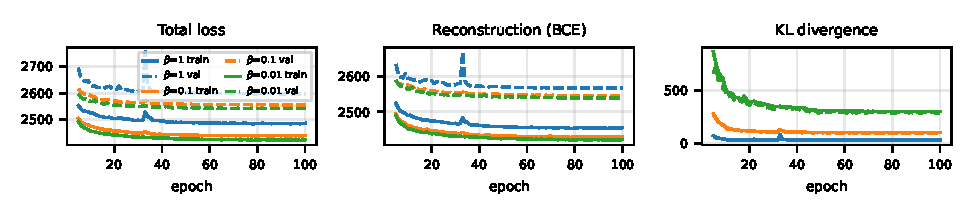
\includegraphics[width=0.94\linewidth]{figures/losses.pdf}
  \caption{Training (solid) and validation (dashed) losses; epochs 1--4 (KL warm-up) omitted.}
  \label{fig:losses}
\end{figure}

\begin{figure}[!b]
  \centering
  \begin{minipage}[c]{0.2\linewidth}\centering
    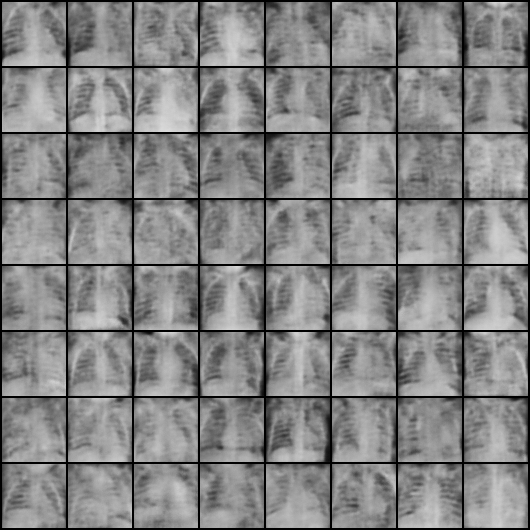
\includegraphics[width=\linewidth]{figures/samples_prior.png}
  \end{minipage}\hfill
  \begin{minipage}[c]{0.2\linewidth}\centering
    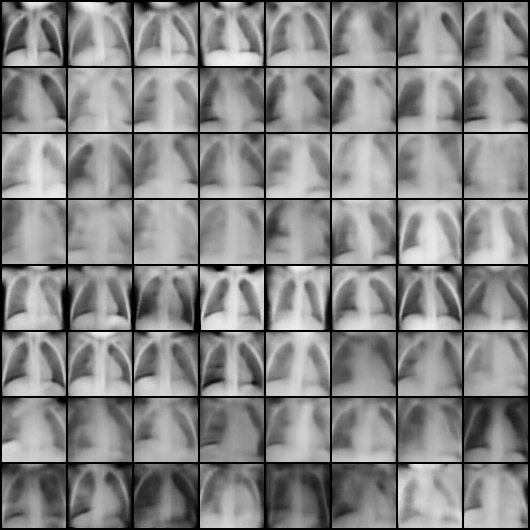
\includegraphics[width=\linewidth]{figures/samples_gmm.png}
  \end{minipage}\hfill
  \begin{minipage}[c]{0.33\linewidth}\centering
    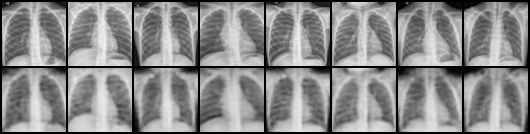
\includegraphics[width=\linewidth]{figures/recon.png}\\[3pt]
    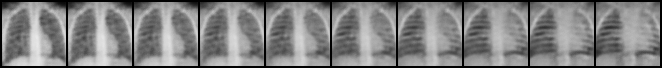
\includegraphics[width=\linewidth]{figures/interp.png}
  \end{minipage}
  \caption{$\beta{=}0.01$ model. Left: prior samples. Middle: GMM samples. Right: test images over their reconstructions (top); latent interpolation from a normal to a pneumonia image (bottom).}
  \label{fig:samples}
\end{figure}

\section{Results}
\textbf{Training.} All runs converge smoothly without overfitting (Fig.~\ref{fig:losses}; train and validation within 5 nats). Smaller $\beta$ lowers validation BCE (2562, 2545, 2539 for $\beta=1,0.1,0.01$) but raises KL (18, 72, 263 nats): codes keep more information and spread further from the prior.

\textbf{Effect of $\beta$.} Reconstruction FID improves steadily as $\beta$ falls (221, 201, 134; Table~\ref{tab:results}). Prior-sample FID is flat from $\beta{=}1$ to $0.1$ (219, 220) and improves only at $\beta{=}0.01$ (185). Presumably a more detailed decoder is offset by codes drifting from $\mathcal{N}(0,I)$, so prior samples land where the decoder was not trained.

\textbf{Effect of the sampling distribution.} GMM sampling helps only for $\beta\le0.1$ (220$\to$207, 185$\to$158). At $\beta{=}1$ the aggregate posterior is already close to $\mathcal{N}(0,I)$ (mean KL 18 nats), so GMM$\approx$prior. At $\beta{=}0.01$ it closes about half of the 50-point gap between prior samples and reconstructions (134). At matched size (GMM@624: 218, 203, 159), GMM samples match reconstructions at $\beta{=}1$ and $0.1$, so there the decoder rather than the sampler limits quality; they trail only at $\beta{=}0.01$ (159 vs.\ 134), where 10 components may not fit the 128-d latents fully. IS of prior samples falls (1.91, 1.84, 1.70) even as FID holds or improves; since ImageNet classes separate these images poorly, we treat IS as uninformative.

\textbf{Augmentation ablation} ($\beta{=}0.01$, rotation $\pm5^\circ$, translation 5\%). FID prior/GMM/recon.\ rises from 185/158/134 to 323/214/206, although validation loss (BCE${}+\beta$KL) is equal (2542). Prior samples of the augmented model have dark borders (mean brightness of the outer 4 pixels: 0.34, vs.\ 0.54 for test images and 0.52 without augmentation), consistent with the decoder learning the black fill of rotated training images. The augmented model's training loss is also 118 nats below validation (2 without), as expected if black corners are easy to reconstruct: augmentation added an artifact without improving generalization.

\textbf{Qualitative.} Prior samples of the $\beta{=}0.01$ model (Fig.~\ref{fig:samples}, left) show chest outlines but are noisier than GMM samples (middle), which have clearer rib cages and lung fields. Reconstructions (right) keep global shape but lose fine rib detail; normal-to-pneumonia interpolation changes smoothly without ghosting. A PCA of test latents shows heavy NORMAL/PNEUMONIA overlap, so classes do not separate. \textbf{Limitations:} one seed per setting, untuned GMM size, no downstream validation.


\clearpage
{\footnotesize
\setlength{\bibsep}{1pt}
\bibliographystyle{plainnat}
\bibliography{references}
}

\end{document}
